\section{Δεύτερη Φάση Πειραμάτων}
\label{sec:experiments_phase2}

Η μέτρηση της ισχύος που καταναλώνει η πλακέτα έγινε ακολουθώντας την παρακάτω μεθοδολογία:
\begin{itemize}
  \item{Από το έγγραφο που περιγράφει τα σχηματικά της πλακέτας \footnote{TK1 Compact Development Module,  602-7R375-0000-D10, σελίδα 27}
    βρέθηκε η αντίσταση (R5C11, 5mΩ) από την οποία περνάει το ρεύμα που παρέχεται από το τροφοδοτικό.}
  \item{Βρέθηκε πάνω στην πλακέτα η θέση της αντίστασης και χρησιμοποιήθηκε ένα
    πολύμετρο για λήψη της τιμής της τάσης στα άκρα της.
    Από την τιμή της αντίστασης και της τάσης στα άκρα της υπολογίζεται το ρεύμα που διέρχεται από αυτήν,
    το οποίο ισοδυναμεί με το ρεύμα που λαμβάνει η πλακέτα από το τροφοδοτικό.}
  \item{Γνωρίζοντας την τιμή της τάσης τροφοδοσίας (12.15Volts) και την τιμή
    του ρεύματος που λαμβάνεται από το τροφοδοτικό, υπολογίζεται η παρεχόμενη στην πλακέτα ισχύ.}
\end{itemize}

Προτού γίνουν μετρήσεις ισχύος, χρησιμοποιήθηκε το εργαλείο \emph{powertop}\footnote{PowerTOP: \url{https://github.com/fenrus75/powertop}},
το οποίο δίνει πληροφορίες σχετικά με τις ενεργοποιημένες μονάδες ενός συστήματος
και την σχετική απόδοσή τους σε κατανάλωση ισχύος (όχι σε τιμές Watt).
Οι πιο κάτω προτάσεις του συγκεκριμένου εργαλείου για το
ενσωματωμένο σύστημα Jetson TK1 λήφθηκαν υπόψη:
\begin{itemize}
  \item{Απενεργοποίηση των ελεγκτών USB (EHCI και xHCI).}
  \item{Ενεργοποίηση λειτουργίας διαχείρισης ισχύος για τον ελεγκτή SATA (SATA link power managment)}
  \item{Ενεργοποίηση λειτουργίας διαχείρισης ισχύος της μονάδας Audio Codec (Audio Codec power managment)}
  \item{Ενεργοποίηση λειτουργίας διαχείρισης ισχύος διαύλου PCIe (PCIe bridge runtime power managment)}
\end{itemize}

Στην συνέχεια μετρήθηκε η τιμή της κατανάλωσης ισχύος της πλακέτας σε κατάσταση αεργίας (idle),
στα $3.4$Watts. Επίσης, ο ανεμιστήρας τον οποίο
διαθέτει το συγκεκριμένο ενσωματωμένο για την ψύξη του TK1 SoC καταναλώνει $0.85$Watts
\footnote{Κατανάλωσης ισχύος του ανεμιστήρα που διαθέτει το Jetson TK1 \url{http://elinux.org/Jetson/Graphics_Performance\#Test_Methodology}}.


Η μεταγλώττιση των δικτύων AlexNet και VGG16 απαιτεί περισσότερη
μνήμη από αυτή που διαθέτει το ενσωματωμένο σύστημα Jetson TK1 (1888MB).
Το πρόβλημα αυτό το αντιμετωπίστηκε προσθέτοντας 1GB μνήμη
\emph{Swap}\footnote{Δημιουργία αρχείου μνήμης swap: \url{http://www.jetsonhacks.com/2014/10/04/creating-swapfile-ubuntu-nvidia-jetson-tk1/}}.

Οι εκδόσεις των εργαλείων λογισμικού που χρησιμοποιήθηκαν
κατά την διάρκεια των πειραμάτων είναι:
\begin{itemize}
  \item{Keras: v1.1.0}
  \item{Theano: v0.9.0-dev3}
  \item{numpy: v1.11.0}
  \item{scipy: v0.19.0-dev0}
\end{itemize}

%%----------------------------------------------------------------------------

\subsection{AlexNet}

Οι παράμετροι των πειραμάτων είναι οι εξής:
\begin{itemize}
  \item{Αριθμός επαναλήψεων: 1000}
  \item{Υπολογιστική μονάδα:}
    \begin{itemize}
      \item{CPU: Αριθμός Νημάτων (1, 2, 4, 8)}
      \item{GPU: Με και χωρίς εκ των προτέρων δέσμευση μνήμης}
    \end{itemize}
\end{itemize}

\begin{figure}[H]
  \centering
  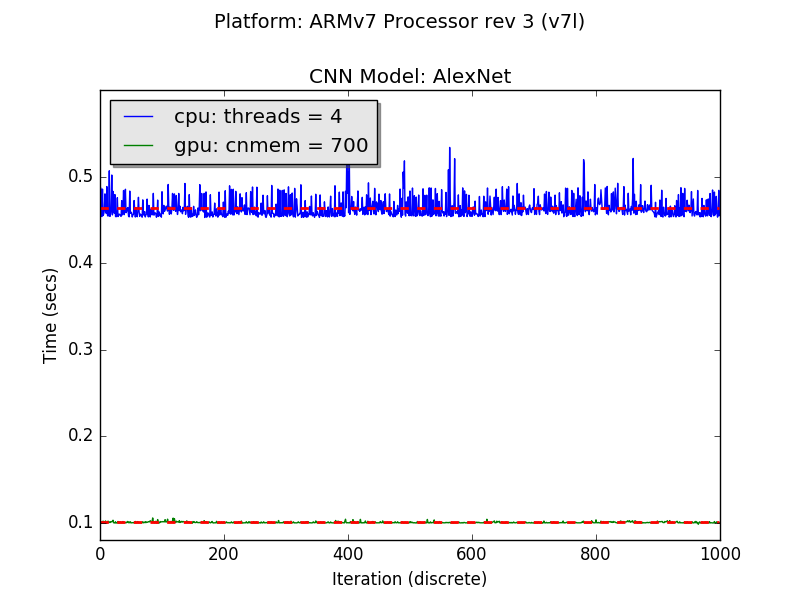
\includegraphics[width=0.8\textwidth]{./images/chapter6/benchmark_alexnet_jetson.png}
  \caption[Χρόνoι εκτέλεσης για το δίκτυο AlexNet στο Jetson TK1]{Χρόνoι εκτέλεσης για το δίκτυο AlexNet στο Jetson TK1}
  \label{fig:alexnet_results_jetson}
\end{figure}

Στον \autoref{tab:alexnet_jetson} παρουσιάζονται τα συγκριτικά αποτελέσματα της
εκτέλεσης τόσο στην μονάδα CPU (με μεταβλητό αριθμό νημάτων), όσο και στην
GPU (με και χωρίς εκ των προτέρων δέσμευση μνήμης).

\begin{table}[H]
  \begin{center}
    \caption{Μετρήσεις πειραμάτων για το δίκτυο AlexNet στο Jetson TK1}
    \label{tab:alexnet_jetson}
    \small
    \begin{tabular}[center]{ | c | c | c | c | c | c | }
      \hline
      \rowcolor{Gray}
      Μονάδα & \# νημάτων & cnmem & Χρόνος εκτέλεσης (sec) & Κατ. Ισχύος (Watts) & Perf/Watt \\
      \hline
      CPU & 1 & N/A & 0.62 & 6.318 & 0.254\\
      CPU & 2 & N/A & 0.4845 & 8.019 & 0.2574\\
      CPU & 4 & N/A & 0.4634 & 10.692 & 0.202\\
      CPU & 8 & N/A & 0.4646 & 10.692 & 0.2013\\
      GPU & N/A & None & 0.1049 & 8.5 & 1.1215\\
      GPU & N/A & 700MB & 0.1 & 8.5 & 1.1764\\
      \hline
    \end{tabular}
  \end{center}
\end{table}


%%----------------------------------------------------------------------------

\subsection{VGG16}

Οι παράμετροι των πειραμάτων είναι οι εξής:
\begin{itemize}
  \item{Αριθμός επαναλήψεων: 100}
  \item{Υπολογιστική μονάδα:}
    \begin{itemize}
      \item{CPU: Αριθμός Νημάτων (1, 2, 4, 8)}
      \item{GPU: Με και χωρίς εκ των προτέρων δέσμευση μνήμης (cnmem)}
    \end{itemize}
\end{itemize}

Στον παρακάτω \autoref{tab:vgg16_jetson} βρίσκονται τα συγκριτικά αποτελέσματα της
εκτέλεσης τόσο στην μονάδα CPU (με μεταβλητό αριθμό νημάτων), όσο και στην
GPU (με και χωρίς εκ των προτέρων δέσμευση μνήμης).

\begin{table}[H]
  \begin{center}
    \caption{Μετρήσεις πειραμάτων για το δίκτυο VGG16 στο Jetson TK1}
    \label{tab:vgg16_jetson}
    \small
    \begin{tabular}[center]{ | c | c | c | c | c | c | }
      \hline
      \rowcolor{Gray}
      Μονάδα & \# νημάτων & cnmem & Χρόνος εκτέλεσης (sec) & Κατ. Ισχύος (Watts) & Perf/Watt \\
      \hline
      CPU & 1 & N/A & 9.431 & 6.318 & 0.0167\\
      CPU & 2 & N/A & 5.4476 &  8.748 & 0.021\\
      CPU & 4 & N/A & 3.6224 & 13.122 & 0.021\\
      CPU & 8 & N/A & 3.6308 & 13.122 & 0.021\\
      GPU & N/A & None & 0.6983 & 11.907 & 0.1207\\
      GPU & N/A & 720MB & 0.5761 & 11.907 & 0.1457\\
      \hline
    \end{tabular}
  \end{center}
\end{table}

Στο \autoref{fig:vgg16_results_jetson} που ακολουθεί, παρουσιάζεται το διάγραμμα
των χρόνων εκτέλεσης στην μονάδα CPU με χρήση τεσσάρων νημάτων και στην μονάδα
GPU με εκ των προτέρων δέσμευση 720MB μνήμης.

%\newpage

\begin{figure}[H]
  \centering
  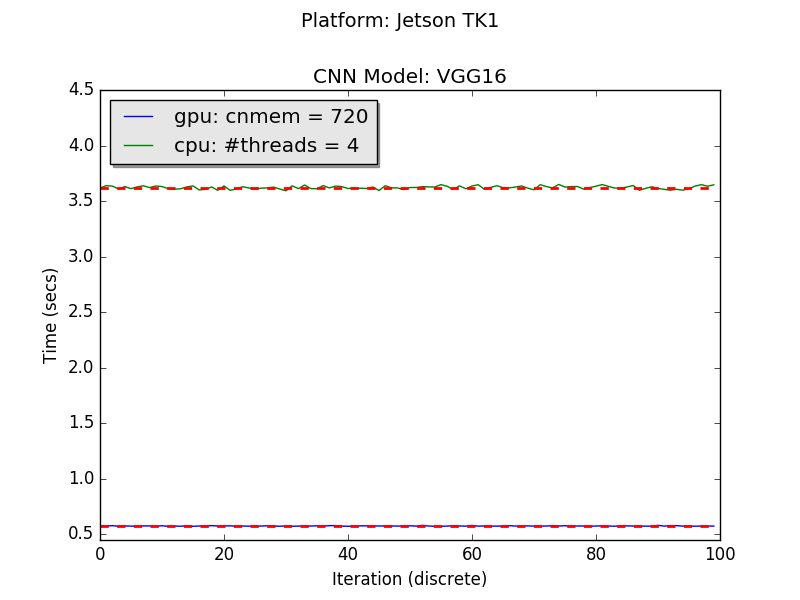
\includegraphics[width=0.8\textwidth]{./images/chapter6/benchmark_vgg16_jetson.png}
  \caption[Χρόνoι εκτέλεσης για το δίκτυο VGG16 στο Jetson TK1]{Χρόνoι εκτέλεσης για το δίκτυο VGG16 στο Jetson TK1}
  \label{fig:vgg16_results_jetson}
\end{figure}


%%----------------------------------------------------------------------------

\subsection{Tiny-YOLO}

Οι παράμετροι των πειραμάτων είναι οι εξής:
\begin{itemize}
  \item{Αριθμός επαναλήψεων: 1000}
  \item{Υπολογιστική μονάδα:}
    \begin{itemize}
      \item{CPU: Αριθμός Νημάτων (1, 2, 4, 8)}
      \item{GPU: Με και χωρίς εκ των προτέρων δέσμευση μνήμης (cnmem)}
    \end{itemize}
\end{itemize}

\begin{table}[H]
  \begin{center}
    \caption{Μετρήσεις πειραμάτων για το δίκτυο Tiny-YOLO στο Jetson TK1}
    \label{tab:yolo_jetson}
    \small
    \begin{tabular}[center]{ | c | c | c | c | c | c | }
      \hline
      \rowcolor{Gray}
      Μονάδα & \# νημάτων & cnmem & Χρόνος εκτέλεσης (sec) & Κατ. Ισχύος (Watts) & Perf/Watt \\
      \hline
      CPU & 1 & N/A & 1.5902 & 6.318 & 0.1\\
      CPU & 2 & N/A & 1.0276 & 8.504 & 0.1144\\
      CPU & 4 & N/A & 0.8137 & 11.9 & 0.103\\
      CPU & 8 & N/A & 0.8126 & 11.9 & 0.1034\\
      GPU & N/A & None & 0.5543 & 8 & 0.2255\\
      GPU & N/A & 400MB & 0.3872 & 8 & 0.323\\
      \hline
    \end{tabular}
  \end{center}
\end{table}

\begin{figure}[H]
  \centering
  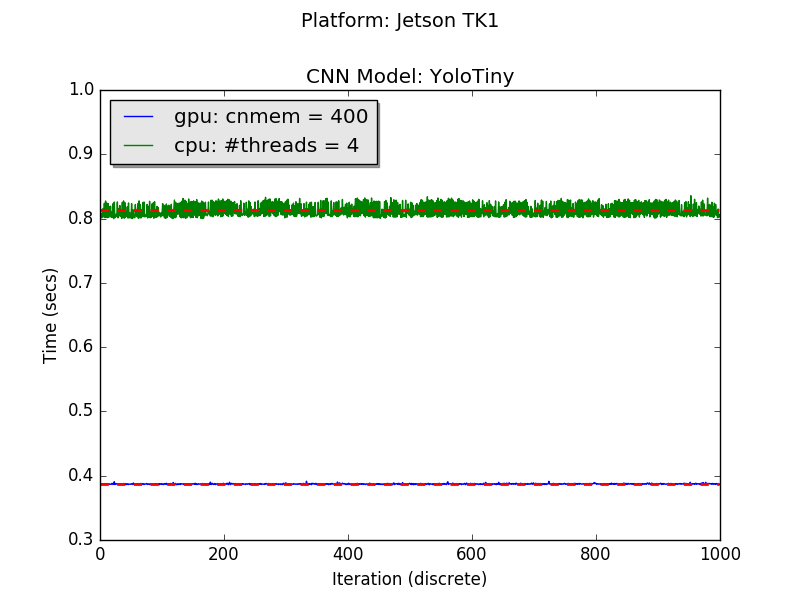
\includegraphics[width=0.8\textwidth]{./images/chapter6/benchmark_yolotiny_jetson.png}
  \caption[Χρόνoι εκτέλεσης για το δίκτυο Tiny-YOLO στο Jetson TK1]{Χρόνοι εκτέλεσης για το δίκτυο Tiny-YOLO στο Jetson TK1}
  \label{fig:yolotiny_results_jetson}
\end{figure}

Ο χρόνος εκτέλεσης της αντίστοιχης υλοποίησης της ερευνητικής ομάδας που
σχεδίασε το δίκτυο Tiny-YOLO μετρήθηκε, για την μονάδα CPU του Tegra K1,
στα 3.475 δευτερόλεπτα (δεν χρησιμοποιούνται νήματα).
Η μέτρηση του χρόνου εκτέλεσης της αντίστοιχης
υλοποίησης στην μονάδα GPU ήταν αδύνατη. Η εκτέλεση στην μονάδα GPU
απαιτούσε περισσότερη μνήμη από αυτή που διαθέτει η πλατφόρμα Jetson TK1 (2GB) και έτσι
το εκτελέσιμο τερματίζει με σφάλμα \emph{CUDA Error: out of memory}.
Ο λόγος που αυτό συμβαίνει μόνο στην περίπτωση εκτέλεσης στην μονάδα GPU
δεν είναι εμφανές. Πιθανόν να οφείλεται σε σφάλμα τύπου διαρροής μνήμης (memory leak).

